% Created 2013-08-08 Thu 17:01
\documentclass[11pt]{article}
\usepackage{fixltx2e}
\usepackage{graphicx}
\usepackage{longtable}
\usepackage{float}
\usepackage{wrapfig}
\usepackage{textcomp}
\usepackage{marvosym}
\usepackage{wasysym}
\usepackage{latexsym}
\usepackage{amssymb}
\usepackage{amstext}
\usepackage{hyperref}
\usepackage[margin=1in]{geometry}
\usepackage{fontspec}
\usepackage{xltxtra}
\usepackage{xunicode}
\usepackage{bidi}
\setmainfont{Linux Libertine}
\tolerance=1000
\author{Mayer Goldberg}
\date{\today}
\title{Arduino Notes}
\hypersetup{
  pdfkeywords={Mayer Goldberg, Department of Computer Science, Ben-Gurion University, Arduino, AVR, C, C++, C/C++, embedded computers, embedded systems, microcomputers, threaded code},
  pdfsubject={},
  pdfcreator={}}
\begin{document}

\maketitle
\tableofcontents


\section{Introduction}
\label{sec-1}

The point of this page is to list all the information \& material I accumulated over the course of working with Arduino. Ideally, this would include code snippets for all the hardware I worked with, so that it would be easier to get started on new projects
\section{Software}
\label{sec-2}

\begin{enumerate}
\item The official Arduino software is located \href{http://arduino.cc/}{here}. It consists of a Java application that includes a compiler for the Arduino platform, a simple IDE, and some functionality for transferring the compiled code to the Arduino board.
\item I'm using Mac OSX 10.6.8. The Arduino board was mis-identified as a
\end{enumerate}

\begin{verbatim}
FT232R USB UART:

  Product ID:	0x6001
  Vendor ID:	0x0403  (Future Technology Devices International Limited)
  Version:	 6.00
  Serial Number:	A1024896
  Speed:	Up to 12 Mb/sec
  Manufacturer:	FTDI
  Location ID:	0x1d100000 / 3
  Current Available (mA):	500
  Current Required (mA):	90
\end{verbatim}

It turns out that I was missing an FTDI driver for emulating a COM port using a USB port. The drivers are available \href{http://www.ftdichip.com/FTDrivers.htm}{here}. 

\section{Basic language reference}
\label{sec-3}

\begin{enumerate}
\item The official language reference is located \href{http://arduino.cc/en/Reference/HomePage}{here}. This includes the basic functions that are available on any Arduino board.

\item Every C/C++ program for the Arduino includes two procedures: \texttt{void setup();} which runs once, upon startup, and \texttt{void loop();} which runs repeatedly.
\end{enumerate}
\section{Hardware}
\label{sec-4}

\subsection{The AVR Microarchitecture}
\label{sec-4-1}

\begin{itemize}
\item The AVR microarchitecture is developed by the \href{http://www.atmel.com/}{Atmel} corporation. All schematics \& data sheets are available through their website.
\item A tutorial on how to program the Arduino in assembly langauge, using the standard \emph{gcc} is available \href{http://www.nongnu.org/avr-libc/user-manual/inline_asm.html}{here}. A post on the same subject can be found \href{http://blog.threebytesfull.com/post/6475041619/arduino-avr-assembly-language}{here}.
\end{itemize}
\subsection{\href{http://dx.com/p/arduino-duemilanove-mega-avr-atmega1280-16au-usb-board-118042}{Arduino Compatible Duemilanove Mega AVR ATmega1280-16AU USB Board}}
\label{sec-4-2}

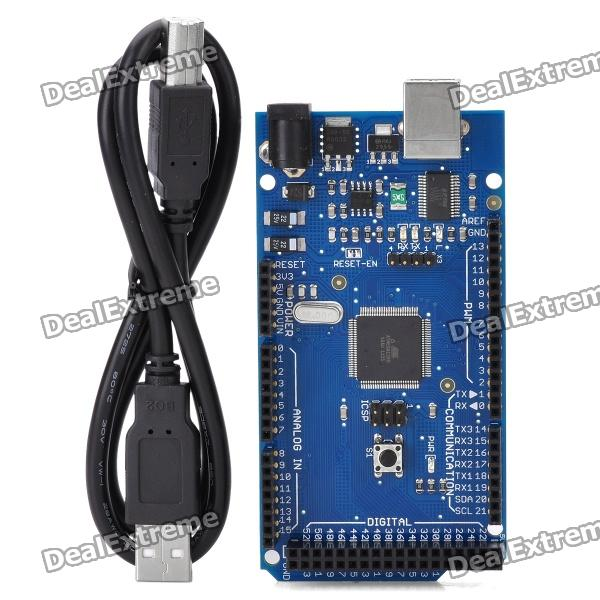
\includegraphics[width=.9\linewidth]{./files/sku_118042_1.jpg}


\begin{itemize}
\item 
\end{itemize}
\subsection{\href{http://dx.com/p/lcd-keypad-shield-for-arduino-duemilanove-lcd-1602-118059}{LCD Keypad Shield for Arduino Duemilanove \& LCD 1602}}
\label{sec-4-3}

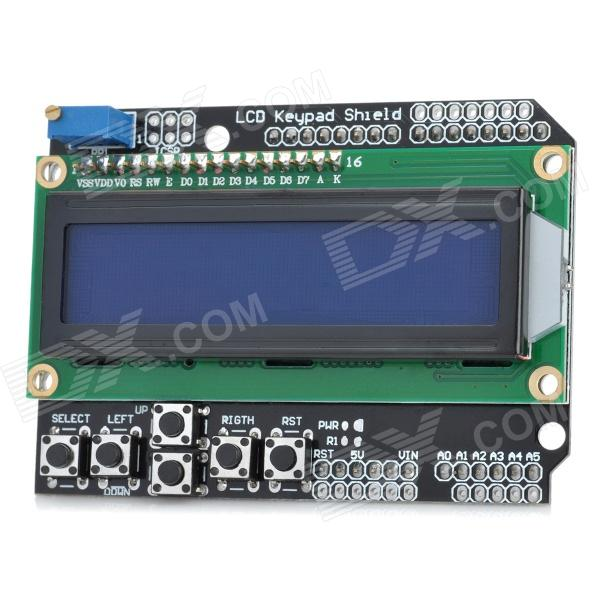
\includegraphics[width=.9\linewidth]{./files/sku_118059_1.jpg}

\subsubsection{Rationale for getting it}
\label{sec-4-3-1}

This is a simple display and some buttons. Enough to display output, read input from the buttons. Can be used to scroll through menu options, etc.
\subsubsection{Programming the LCD Keypad}
\label{sec-4-3-2}

\begin{itemize}
\item \href{http://www.dfrobot.com/wiki/index.php?title=Arduino_LCD_KeyPad_Shield_(SKU:_DFR0009)}{Manufacturer \& data}
\item It was kind of disappointing to learn that the LCD Keypad only permits 8 glyphs to be defined (0-7), so that the full range of Hebrew cannot be defined. Clearly, someone has already thought of this possibility, since the LiquidCrystal library supports writing in either \emph{left-to-right} or \emph{right-to-left}, controllable via the \texttt{lcd.leftToRight();} and \texttt{lcd.rightToLeft();} commands.
\end{itemize}

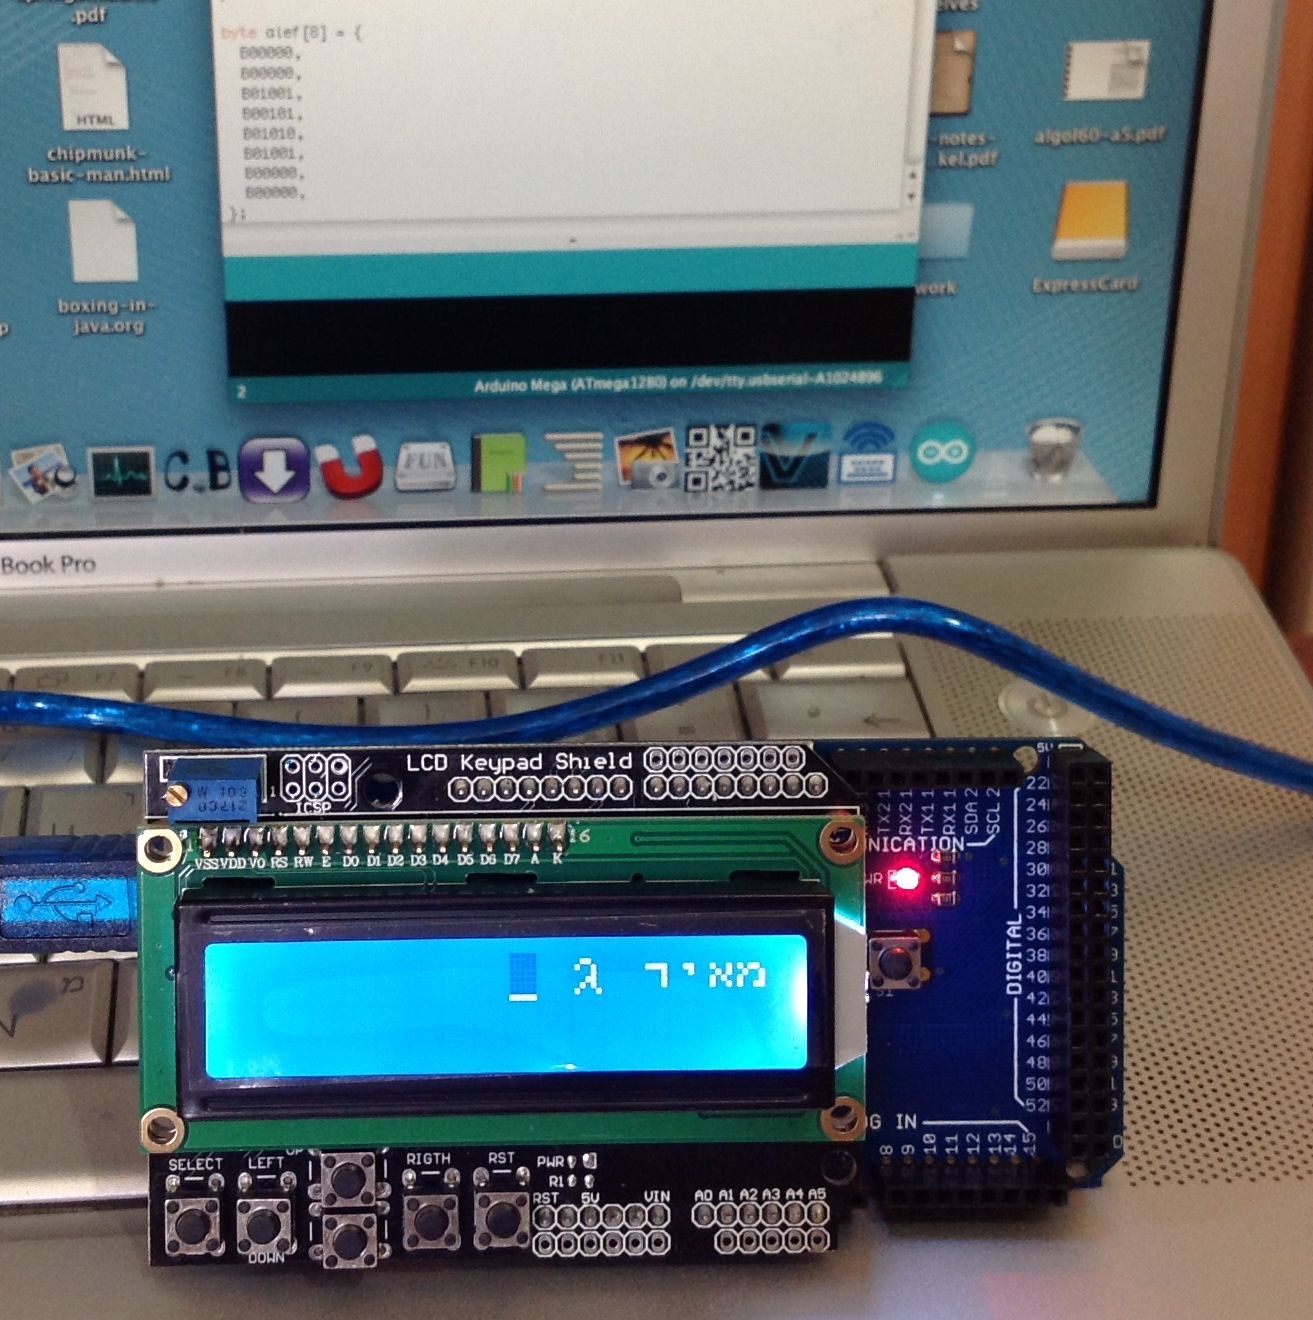
\includegraphics[width=.9\linewidth]{./files/lcd-rtl.jpg}
\subsection{\href{http://dx.com/p/arduino-diy-part-buzzer-module-black-138322}{Arduino Compatible Passive Speaker Buzzer Module - Black}}
\label{sec-4-4}

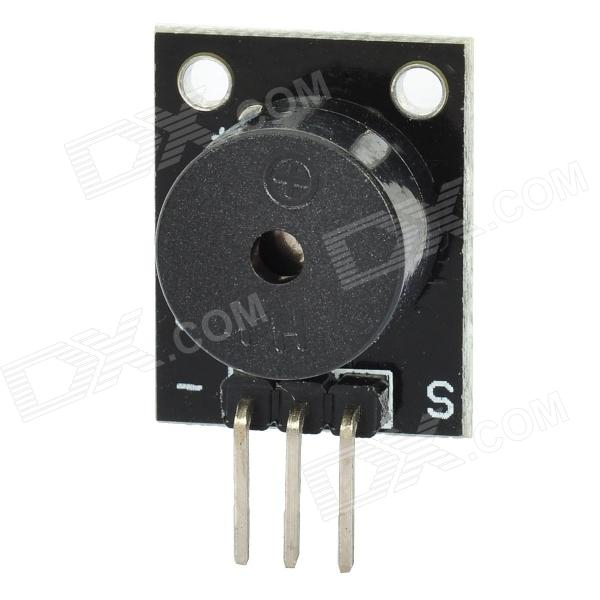
\includegraphics[width=.9\linewidth]{./files/sku_138322_1.jpg}

\begin{itemize}
\item The buzzer comes with 3 pins, whereas most buzzers I see on various Arduino tutorials come with only two. I have no idea what the third pin is like. One of the pins is marked with a minus sign '\textbf{-}', so it is plugged into \textbf{GND} on the Arduino board. This makes the second (middle) pin fit into \textbf{13}, and the third pin fit into \textbf{12}. Attempts to use \textbf{13} failed. Attempts to use \textbf{12} succeeded beautifully.
\item To operate the buzzer, the \texttt{void init();} function must contain an initialization to the buzzer output pin, which in this case is \textbf{12}. Ideally, this should be set using a C macro to abstract the number of the pin: \texttt{pinMode(BUZZER\_OUTPUT, OUTPUT);}. The \texttt{void loop();} function should contain
\end{itemize}
\subsection{\href{http://dx.com/p/arduino-1-6-lcd-display-screen-for-nokia-5110-red-silver-140226}{Arduino Compatible 1.6" LCD Nokia 5110 LCD Module with White Backlit - Red + Silver}}
\label{sec-4-5}
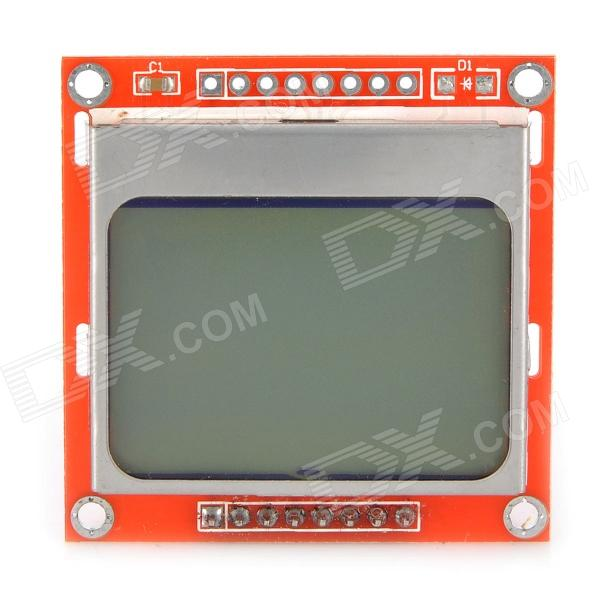
\includegraphics[width=.9\linewidth]{./files/sku_140226_1.jpg}

\begin{itemize}
\item Spec \& technical details are \href{https://www.sparkfun.com/products/10168}{here}.
\end{itemize}
\subsection{\href{http://dx.com/p/mcu-extension-4-x-4-16-key-matrix-keyboard-module-for-arduino-green-147734}{MCU Extension 4 x 4 16-Key Matrix Keyboard Module for Arduino - Green}}
\label{sec-4-6}
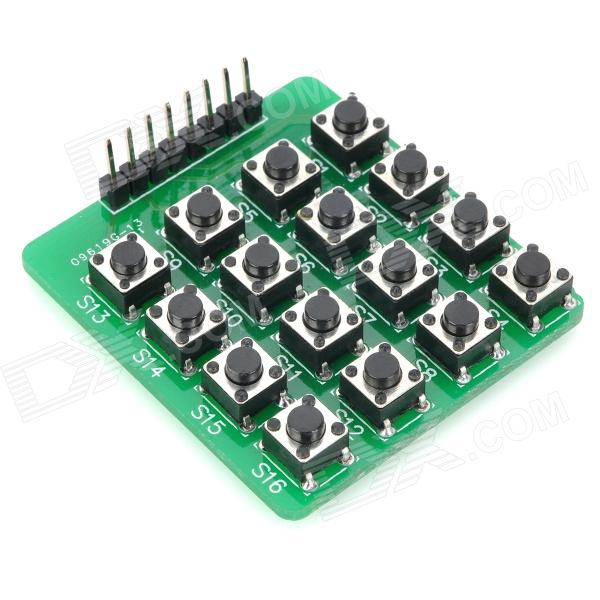
\includegraphics[width=.9\linewidth]{./files/sku_147734_1.jpg}
\subsection{\href{http://dx.com/p/sd-card-reading-writing-module-for-arduino-148784}{SD Card Reading Writing Module for Arduino}}
\label{sec-4-7}
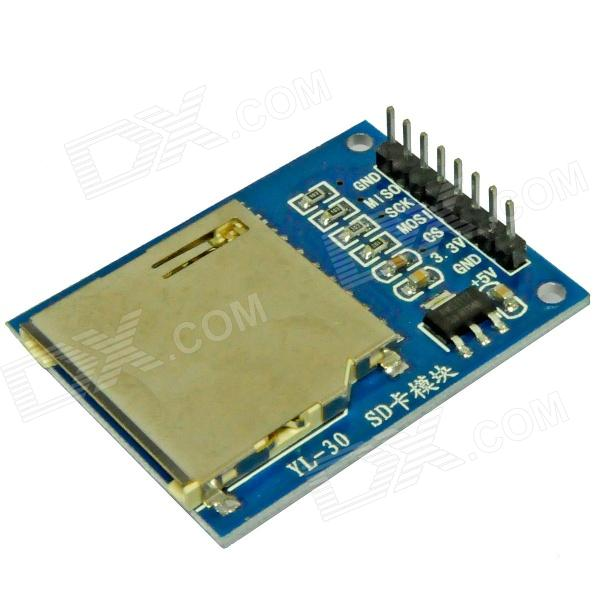
\includegraphics[width=.9\linewidth]{./files/sku_148784_1.jpg}

\subsubsection{Rationale for getting it}
\label{sec-4-7-1}

The SD card is an inexpensive (US\$2.70) way of storing information for or by the Arduino. This memory is non-volatile, and the API for the SD card comes with functions for creating directories, reading, writing, and deleting files, etc.

Because memory is scarce on the Arduino, large amounts of data, structured or unstructured, can be stored on an SD card and used by Arduino programs. 

For \emph{threaded code}, this offers a simple and effective way to store code \& data, so that the only native code need be the \emph{address interpreter}. The \emph{control stack}, the \emph{data stack}, the \emph{dictionary}, etc, can all reside as files on the SD card, and accessed via random-access IO operations.
\subsection{\href{http://dx.com/p/ds1302-real-time-clock-module-with-battery-cr2032-126453}{DS1302 Real Time Clock Module with Battery CR2032}}
\label{sec-4-8}

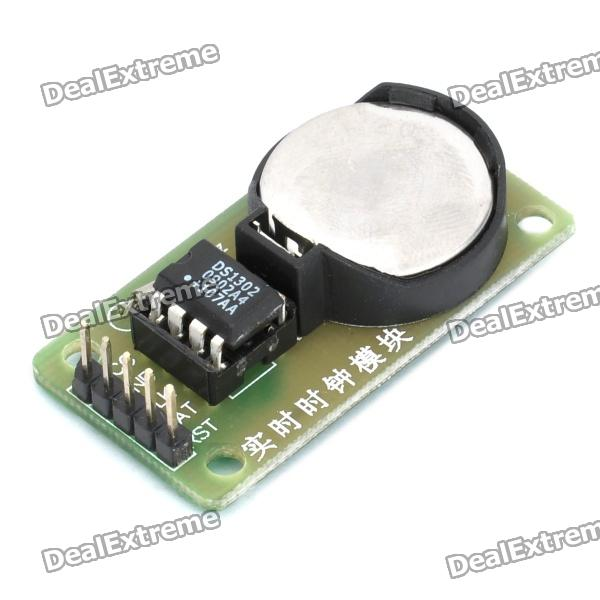
\includegraphics[width=.9\linewidth]{./files/sku_126453_2.jpg}

\subsubsection{Rationale for getting it}
\label{sec-4-8-1}

The Arduino does not come with a built-in, real-time clock (!). This means that it cannot tell time. For any project that requires keeping time (alarm clock, etc) you want to get a real time clock shield. The beauty of this unit is that it has a very simple API for setting \& getting the time, and the battery will let it keep the time for several years, independently of the power supply to the main board.
\subsection{\href{http://dx.com/p/5v-3-2-lcd12864-screen-module-with-backlit-yellow-green-screen-english-word-stock-121820}{5V 3.2" LCD12864 Screen Module with Backlit (Yellow \& Green Screen/English Word Stock)}}
\label{sec-4-9}
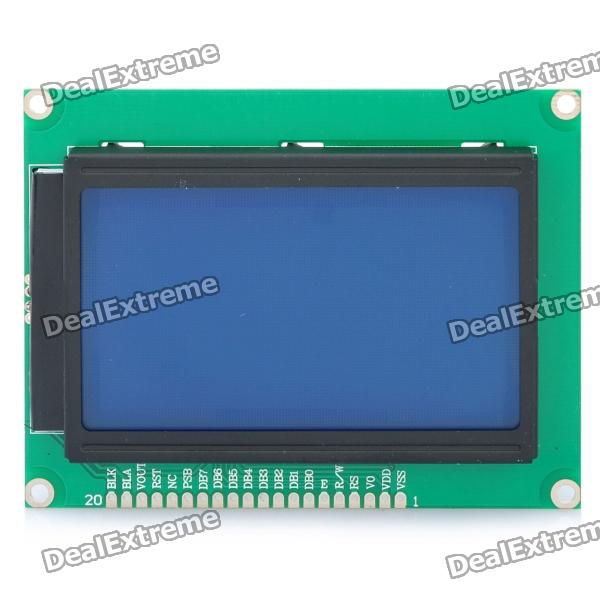
\includegraphics[width=.9\linewidth]{./files/sku_121820_1.jpg}
\subsection{TM1638 LED Button(8-Bit Digital Tube+8 LED+8 Key) For Arduino ARM STM32 A104}
\label{sec-4-10}
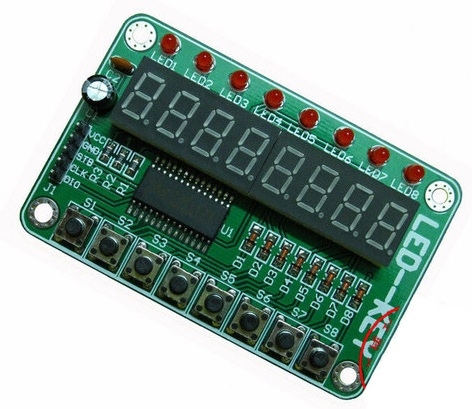
\includegraphics[width=.9\linewidth]{./files/led-shield.jpg}

\begin{itemize}
\item Specs in English can be found \href{http://tronixstuff.wordpress.com/2012/03/11/arduino-and-tm1638-led-display-modules/}{here}.
\end{itemize}
\subsection{Cables, Connectors, etc.}
\label{sec-4-11}

The wires that are used to connect pins on PCB are called \emph{Dupont jumper wires}. The pins are called \emph{pin headers}. 

\begin{itemize}
\item General: \href{http://dx.com/s/electronic+pins.html?category=410&PageSize=60}{Pins}
\item \href{http://dx.com/p/male-to-female-dupont-breadboard-jumper-wires-for-arduino-40-piece-pack-20cm-length-146935}{Male-to-female jumper wires}
\item \href{http://dx.com/p/arduino-compatible-breadboard-jumper-wires-8-20cm-68-cable-pack-142221}{Male-to-male jumper wires}
\item \href{http://dx.com/p/arduino-dupont-4-pin-female-to-female-extension-wire-cable-40cm-10-piece-pack-140526}{Female-to-female jumper wires}
\item \href{http://dx.com/p/single-row-40-pin-2-00mm-pitch-pin-headers-200-piece-pack-139825}{Pin headers} for soldering to a PCB
\item \href{http://dx.com/p/840-point-solderless-breadboard-118355}{840-pin solderless breadboard}. Comes with notches and grooves on the side, so that any number of similar breadboards can be fitten to form a longer and wider work area.
\end{itemize}

\section{Hardware I need to get}
\label{sec-5}

\begin{enumerate}
\item A GPS fence
\item A touch screen
\item Connectors to connect shields to the main board
\item A bluetooth shield
\item An FM radio shield
\item \href{http://dx.com/p/new-version-pro-mini-atmega328p-microcontroller-board-white-173878}{New Version Pro Mini Atmega328P Microcontroller Board - White}
\item \href{http://dx.com/p/efcom-pro-wireless-850-900-1800-1900mhz-gprs-gsm-module-w-antenna-white-173749}{EFCom Pro Wireless 850/900/1800/1900MHz GPRS/GSM Module w/ Antenna - White}
\item \href{http://dx.com/p/jy-mcu-arduino-bluetooth-wireless-serial-port-module-104299}{JY-MCU Arduino Bluetooth Wireless Serial Port Module}
\item \href{http://dx.com/p/usb-host-shield-2-0-board-166217}{USB Host Shield 2.0 Board}
\item \href{http://dx.com/p/2-4ghz-nrf24l01-wireless-communication-module-for-arduino-green-2-pcs-149255}{2.4GHz NRF24L01+ Wireless Communication Module for Arduino - Green (2 PCS)}
\item \href{http://dx.com/p/diy-colorful-lcd-shield-nokia-6100-expansion-board-white-171914}{DIY Color LCD Shield Nokia 6100 Expansion Board - White}
\item \href{http://www.ebay.com/itm/130839929399?ssPageName=STRK:MEWNX:IT&_trksid=p3984.m1497.l2649}{New Version Pro Mini Atmega328P Microcontroller Board - White}
\end{enumerate}
\section{Miscellaneous, unsorted, open questions}
\label{sec-6}
\begin{enumerate}
\item Connecting the Arduino board
\begin{enumerate}
\item What buttons are on the board, and which ones can I control?
\item How do I write to the equivalent of the console? --- something that can be recognized from the Arduino IDE.
\end{enumerate}
\item Connecting the LCD keypad
\begin{enumerate}
\item Recognising the buttons for press \& release
\item Writing bitmaps to the LCD
\end{enumerate}
\item Connecting to the SD card
\begin{enumerate}
\item What is the max file size?
\item How many open files can one have simultaneously?
\end{enumerate}
\end{enumerate}
\end{document}